\documentclass[notes=hide]{beamer}
\usepackage{graphicx}
\usetheme{Warsaw}
\title{Improving dynamic allocation in cluster schedulers}
\author{Inigo Mediavilla}
\institute[Inst.]{\large{UPMC} \\
\includegraphics[height=1cm,width=2cm]{viadeo.jpg}}
\date\today
%%\setbeamertemplate{note page}[plain]
\setbeamertemplate{page}[plain]

\graphicspath{ {./images/} }

\begin{document}

  \begin{frame}
  \titlepage
  \end{frame}
  
  \note{}

  \begin{frame}
    \frametitle{Scheduling}
    \begin{definition}{Scheduling:}
    planning the execution of a set of computations that
    are called jobs in an execution environment with a limited amount
    of resources.
    \end{definition}
    \begin{definition}{Framework:}
    Application trying to run computations in the cluster.
    \end{definition}
  \end{frame}

  \note{}

  \begin{frame}
    \frametitle{Scheduling}
    \begin{itemize}
      \item Why does it matter?
      \begin{itemize}
        \item Growing datacenters for big companies (Google, Yahoo!,
          Facebook, Amazon)
        \item Small and Medium sized companies own more clusters (in
          the cloud or physically)  
        \item Increasing popularity of distributed processing
      \end{itemize}
    \end{itemize}
    \begin{itemize}
      \item Why is it difficult?
        \begin{itemize}
          \item Increasing size of clusters
          \item Growing number of jobs to run
          \item Jobs are more sensitive to scheduling delays
          \item Diversity of scheduling needs
          \item Need to ensure fairness
        \end{itemize}
     \end{itemize}
  \end{frame}

  \note{}

  \begin{frame}
    \frametitle{Research Question}
    \begin{itemize}
      \item
        How to provide a scheduler that scales well, is flexible to
        support diverse strategies and is capable of ensuring a fair
        repartition?
    \end{itemize}
  \end{frame}

  \note{}


  \begin{frame}
    \frametitle{Summary}
    \begin{itemize}
      \item[A] Analysis of existing solutions
      \item[B] Propositions
        \begin{enumerate}
          \item Adding fairness and datalocality to Omega
          \item Simulating Optimistic locking with Mesos
        \end{enumerate}
      \item[C] Conclusions and further work
    \end{itemize}
  \end{frame}

  \note{}

  \begin{frame}
    \frametitle{Analysis of existing solutions}
    \begin{block}{Section A}
    \begin{itemize}
         \item Analysis of existing solutions
    \end{itemize}
     \end{block}
  \end{frame}

  \begin{frame}
    \frametitle{Analysis of existing solutions}
    \begin{enumerate}
      \item Centralized Scheduler (single-path or multi-path)
      \item Static partitioning
      \item Two level Schedulers (i.e. Mesos)
      \item Optimistic locking (i.e. Omega)
    \end{enumerate}
  \end{frame}

  \note{}

  \begin{frame}
    \frametitle{Centralized Scheduler}
    \begin{columns}[T]
       \begin{column}{.5\textwidth}
        \begin{block}{Pros/Cons}
            \begin{itemize}
              \item[+] Initially simple
              \item[+] Efficient policies with few frameworks
              \item[-] Scalability problems: scheduler is a bottleneck
              \item[-] Head of line blocking (even with multi-path)
              \item[-] Can't deal with different scheduling needs
            \end{itemize}
   % Your text here
        \end{block}
       \end{column}
       \begin{column}{.6\textwidth}
   % Your image included here
         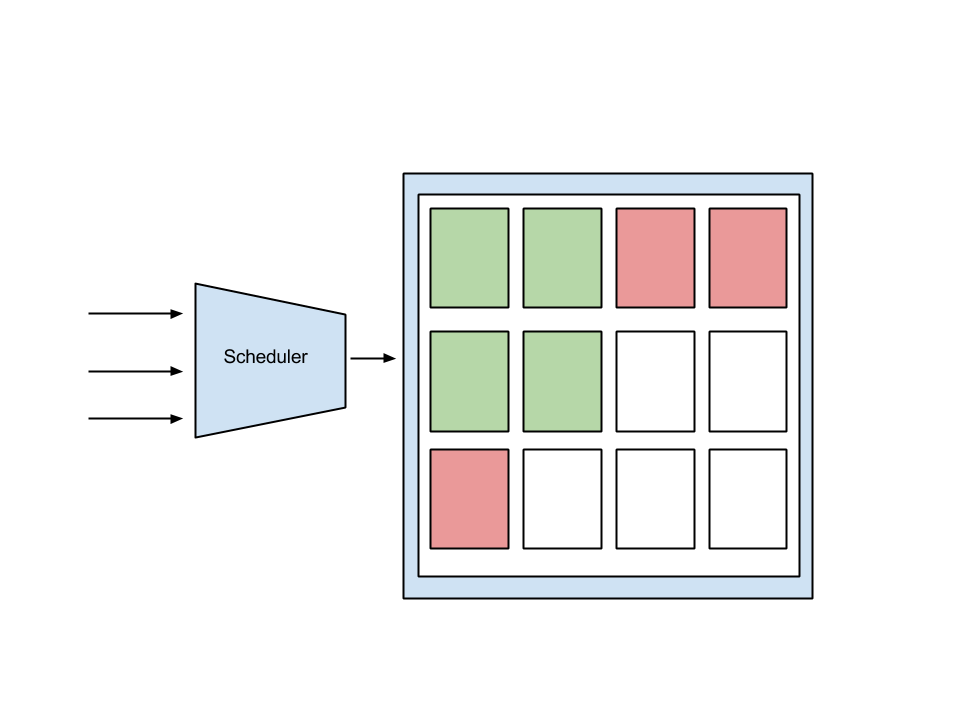
\includegraphics[trim = 0mm 0mm 50mm 0mm,clip,scale=0.20,natwidth=960,natheight=720]{CentralizedScheduler.png}
       \end{column}
     \end{columns}
  \end{frame}

  \note{}

  \begin{frame}
    \frametitle{Static partitioning}
       \begin{columns}[T]
       \begin{column}{.5\textwidth}
        \begin{block}{Pros/Cons}

            \begin{itemize}
              \item[+] Frameworks can schedule the way they want 
              \item[+] No possibility of conflicts
              \item[-] Really inefficient use of the cluster
            \end{itemize}
        \end{block}
        \end{column}
        \begin{column}{.6\textwidth}
         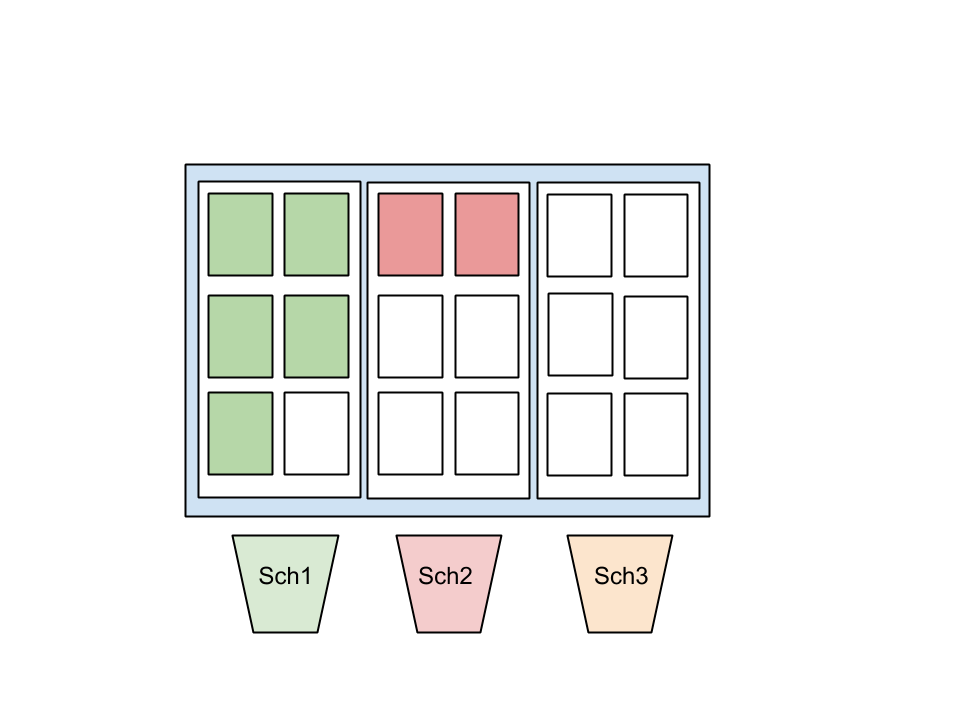
\includegraphics[trim = 40mm 30mm 30mm 40mm,clip,scale=0.30,natwidth=960,natheight=720]{StaticPartitioning-slides.png}
        \end{column}
      \end{columns}
  \end{frame}

  \note{}

  \begin{frame}
    \frametitle{Two-Level Scheduler}
    \begin{definition}
      A central scheduler offers the available resources to
      the frameworks that can accept them and launch tasks
      with them. (Hindman et al.)  
    \end{definition}
    \begin{itemize}
      \item Resources are dynamically allocated
      \item Frameworks schedule tasks the way they want
        with the resources they get
    \end{itemize}
  \end{frame}

  \note{}

  \begin{frame}
    \frametitle{Two-Level Scheduler}
       \begin{columns}[T]
       \begin{column}{.5\textwidth}
        \begin{block}{Pros/Cons}
            \begin{itemize}
              \item[+] Resources are no longer compartimented
              \item[+] No possibility of conflicts
              \item[-] Long frameworks slow down the cluster
              \item[-] Two frameworks hoarding resources can provoke a deadlock
            \end{itemize}
        \end{block}
        \end{column}
        \begin{column}{.6\textwidth}
         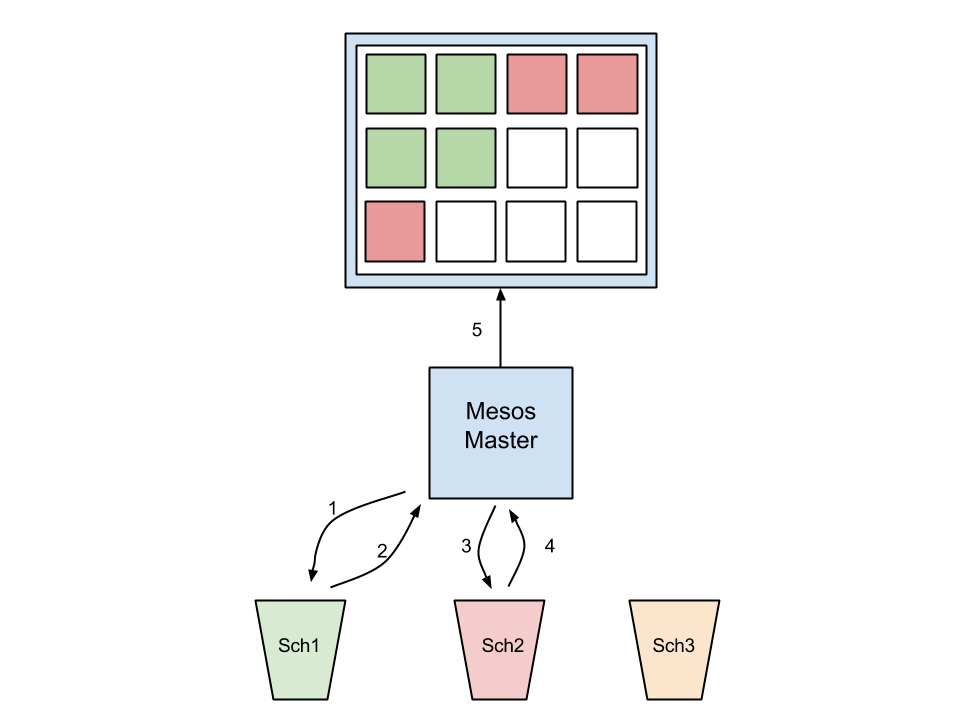
\includegraphics[trim = 50mm 0mm 0mm 0mm,clip,scale=0.30,natwidth=960,natheight=720]{TwoLevel-slides.png}
        \end{column}
      \end{columns}
  \end{frame}

  \note{}

  \begin{frame}
    \frametitle{Omega Scheduler}
    \begin{definition}
      Every framework knows the state of the cluster that
      is updated only by the scheduler. The scheduler's role
      is just to mediate when conflict happens and share
      the state of the cluster with the frameworks when updates
      happen.(Schwarzkopf et al.)
    \end{definition}
  \end{frame}

  \note{}


  \begin{frame}
    \frametitle{Omega Scheduler}
       \begin{columns}[T]
       \begin{column}{.5\textwidth}
        \begin{block}{Pros/Cons}
            \begin{itemize}
              \item[+] Frameworks don't lock
              \item[+] Slow scheduling don't block
              \item[+] Frameworks can be elastic 
              \item[-] No implementation 
              \item[-] No fairness 
            \end{itemize}
         \end{block}
       \end{column}
       \begin{column}{.6\textwidth}
         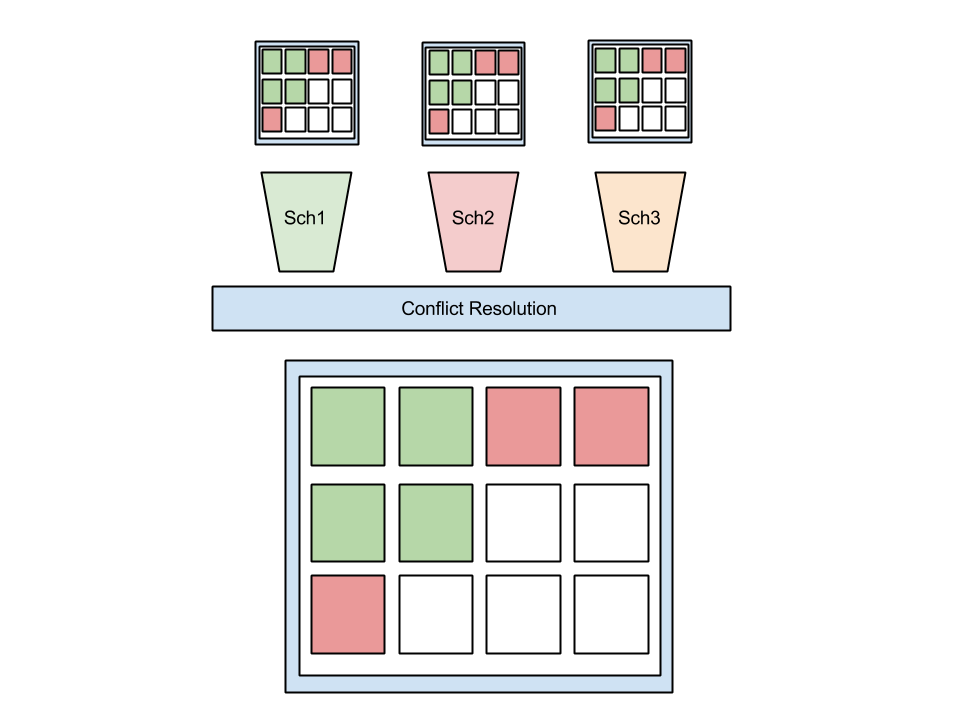
\includegraphics[trim = 50mm 0mm 0mm 0mm,clip,scale=0.30,natwidth=960,natheight=720]{Omega.png}
       \end{column}
       \end{columns}
  \end{frame}

  \note{}


  \begin{frame}
    \frametitle{Propositions}
    \begin{block}{Section B}
    \begin{itemize}
         \item Propositions
    \end{itemize}
     \end{block}
  \end{frame}

  \begin{frame}
    \frametitle{Propositions}
    Prototype implementations of Mesos and Omega
    \begin{enumerate}
        \item Adding fairness and datalocality to Omega
        \item Simulation optimistic locking with Mesos 
    \end{enumerate}
  \end{frame}

  \note{

    \begin{itemize}
        \item Omega's is first proposed implementation
        \item Allow to:
        \begin{itemize}
          \item Study the two different models
          \item Spot similarities - Propose common models (e.g
            cross-model simulations)
          \item Test features
          \item Test performance
          \item Test general solutions in the two models 
        \end{itemize}
        \item Simplifications
          \begin{itemize}
            \item Frameworks are really simple internal processes (no
              different scheduling needs emulated)
            \item Tasks aren't run distributedly (just in their own thread)
            \item No high volumes of traces run against the prototypes
          \end{itemize}
    \end{itemize}
  }

  \begin{frame}
    \frametitle{Adding fairness and datalocality to Omega}
      \begin{center}
      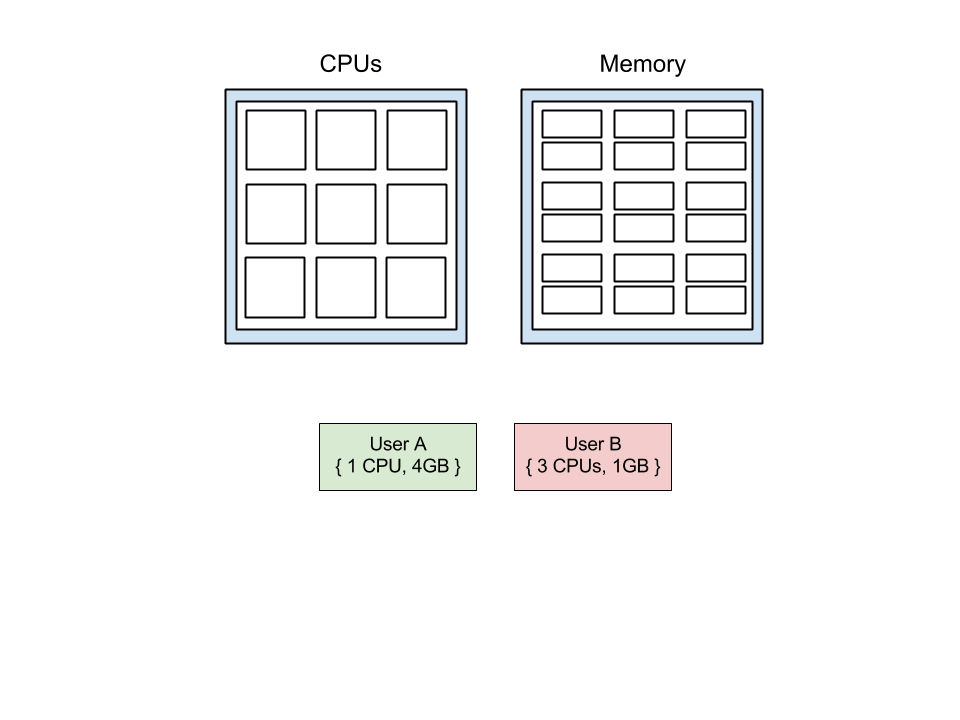
\includegraphics[trim = 50mm 80mm 50mm 17mm,clip,scale=0.34,natwidth=960,natheight=720]{DRF-Process(1).png}
      \end{center}
      \begin{itemize}
        \item Dominant Resource A: CPU (1/9) Mem (4/18) $\Rightarrow$ Mem
        \item Dominant Resource B: CPU (3/9) Mem (1/18) $\Rightarrow$ CPU
      \end{itemize}
  \end{frame}

  \begin{frame}
    \frametitle{Adding fairness and datalocality to Omega}
    Used DRF (Ghodsi et al.)
    \begin{itemize}
      \item The dominant resource (DR) represents the bottleneck
      \item The idea is to give an equivalent \% of the DR
      \item A task whose \% of DR is bigger gets less tasks
    \end{itemize}
  \end{frame}

  \note{}

  \begin{frame}
    \frametitle{Adding fairness and datalocality to Omega}
      \includegraphics[trim = 50mm 0mm 0mm 10mm,clip,scale=0.45,natwidth=960,natheight=720]<1>{DRF-Process(1).png}
      \includegraphics[trim = 50mm 0mm 0mm 10mm,clip,scale=0.45,natwidth=960,natheight=720]<2>{DRF-Process(2).png}
      \includegraphics[trim = 50mm 0mm 0mm 10mm,clip,scale=0.45,natwidth=960,natheight=720]<3>{DRF-Process(3).png}
      \includegraphics[trim = 50mm 0mm 0mm 10mm,clip,scale=0.45,natwidth=960,natheight=720]<4>{DRF-Process(4).png}
      \includegraphics[trim = 50mm 0mm 0mm 10mm,clip,scale=0.45,natwidth=960,natheight=720]<5>{DRF-Process(5).png}
      \includegraphics[trim = 50mm 0mm 0mm 10mm,clip,scale=0.45,natwidth=960,natheight=720]<6>{DRF-Process(6).png}
  \end{frame}
  \note{}

  \begin{frame}
    \frametitle{Adding fairness and datalocality to Omega}
    \begin{itemize}
      \item What is datalocality?
      \item Fairness algorithms attemp against datalocality
      \item How to have datalocality + fairness?
      \begin{itemize}
        \item Delay scheduling (et al.)
      \end{itemize}
    \end{itemize}
  \end{frame}

  \note{}

  \begin{frame}
    \frametitle{Simulating optimistic locking with Mesos}
       \begin{columns}[T]
       \begin{column}{.4\textwidth}
        \begin{block}{Simulation}
            \begin{itemize}
              \item How does it work?
              \item Pros/Cons
              \item Mixed strategy
            \end{itemize}
         \end{block}
       \end{column}
       \begin{column}{.65\textwidth}
         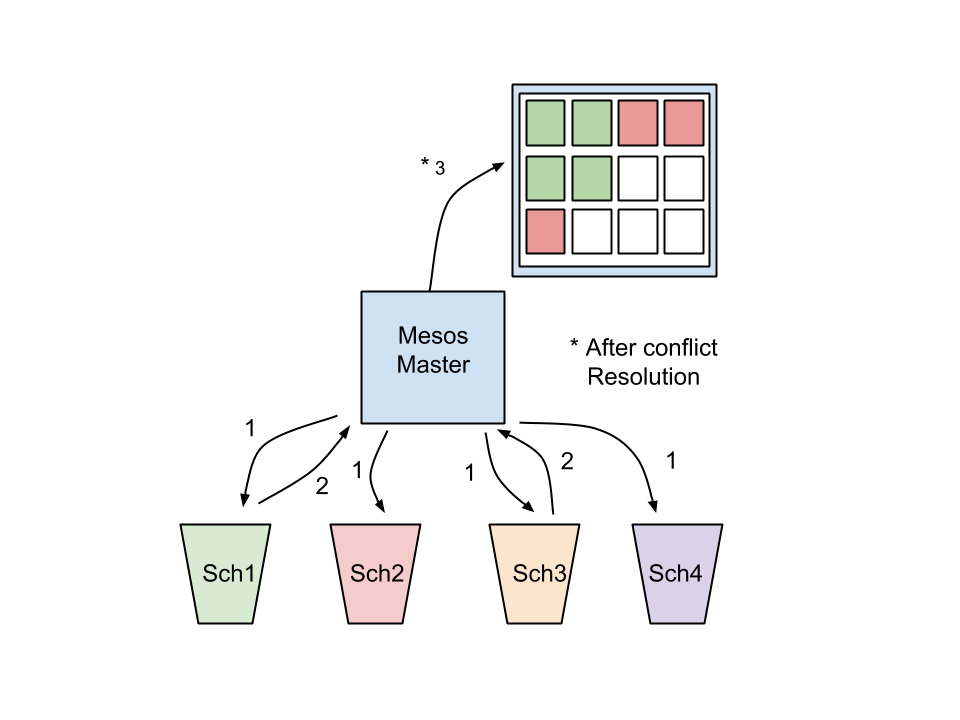
\includegraphics[trim = 63mm 20mm 0mm 20mm,clip,scale=0.35,natwidth=960,natheight=720]{MesosOptimisticLocking-slides.png}
       \end{column}
       \end{columns}
  \end{frame}


  \note{
    It is an improvement over Mesos that allows to emulate the
    optimistic locking model of Omega in Mesos.

    It works by changing the usual model of Mesos where only one
    resource is offered to one framework at a time, to a model where
    available resources are offered to all frameworks at the same
    time this way avoiding the problems of pessimistic locking.

    This improvement would allow with a few simple modifications of
    Mesos to emulate Omega in Mesos, however it has some limitations
    when compared with Omega in terms of efficiency. While in Omega
    only if a framework wants resources it will make a demand, in this
    model frameworks are constantly communicating with the Master even
    if they are not interested in running a task.
    
    Despite it's limitations this model its really interesting and we
    would like it with a proof of concept implementation of it because
    it allows not having to decide between the Omega or the Mesos
    model. It allows a mixed workload where a part of the cluster runs
    with Mesos normal configuration and the rest with an Omega-like
    approach, making Mesos adapt better to any kind of workload.

  }

  \begin{frame}
    \frametitle{Conclusions and further work}
    \begin{block}{Section C}
    \begin{itemize}
         \item Conclusions and futher work 
    \end{itemize}
     \end{block}
  \end{frame}


  \begin{frame}
    \frametitle{Conclusions}
    \begin{itemize}
      \item Prototype implementations of Mesos and Omega 
      \begin{itemize}
        \item Useful to test and understand the models
        \item Help to come up with contributions
       \end{itemize}
       \item Proof that is feasible  a
         production-ready Omega
        \begin{itemize}
          \item Simplicity of the model
          \item Addition of fairness and datalocality
        \end{itemize}
       \item Meanwhile Mesos with optimistic locking as an alternative 
        \begin{itemize}
          \item Has some limitations 
          \item But supports mixed strategies 
        \end{itemize}

    \end{itemize}
  \end{frame}

  \note{
    The prototype implementations of the two most important models has
    proved really useful as a way to understand better the
    implications of the two different models (Mesos y Omega) and has
    allowed us to experiment with new features and come up with contributions.

    The addition of an algorithm to manage fairness and datalocality
    in Omega and the implementation in a prototype its really
    promising because it shows that it is feasible to define a in the
    mid term a production ready implementation of Omega that could be
    opensourced and compete with Mesos.

    In the short term we've proposed a way to simulate Omega in Mesos
    what could bring quickly some of the benefits of the model behind
    Omega to a fully featured cluster scheduler like Mesos.

    

  }

  \begin{frame}
    \frametitle{Further work}
    \begin{itemize}
      \item Add optimistic locking to Mesos
      \item Further test contributions 
      \begin{itemize}
        \item Test against google's traces
       \end{itemize}
      \item Add features to Omega prototype
      \begin{itemize}
        \item Provide isolation, failover, a nice API
        \item Add documentation
        \item Add easy setup of a cluster
       \end{itemize}
      \item Improve DRF
      \begin{itemize}
        \item Add weighted DRF
        \item Simpler datalocality aware DRF
       \end{itemize}

    \end{itemize}
  \end{frame}

  \note{

  }

  \begin{frame}
    \frametitle{Questions}
    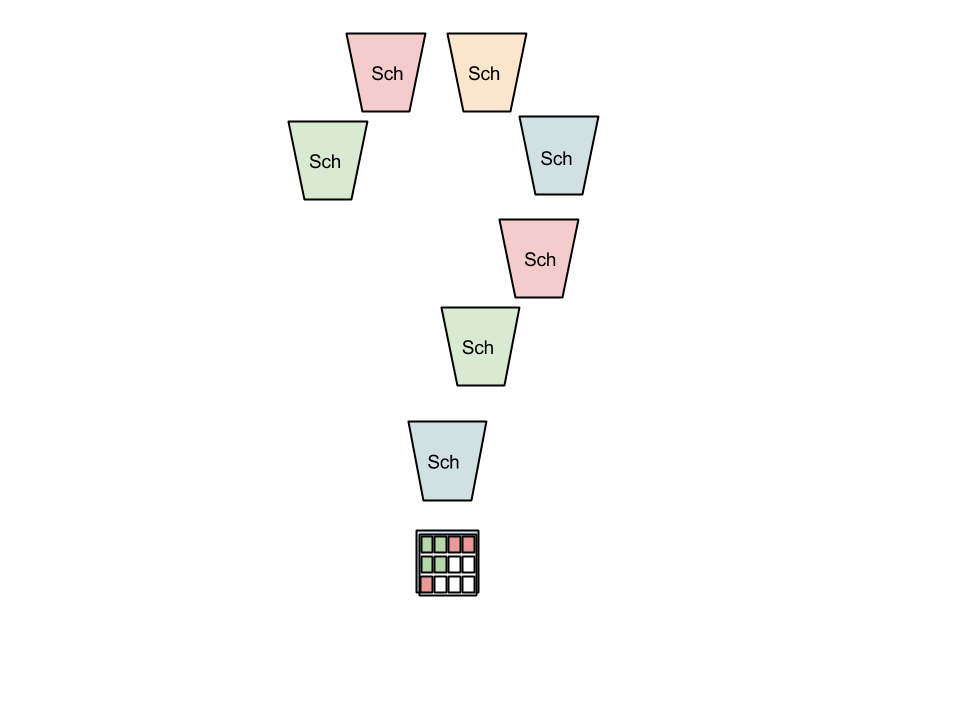
\includegraphics[trim = 0mm 0mm 25mm 0mm,clip,scale=0.35,natwidth=960,natheight=720]{Question.png}
  \end{frame}


\end{document}
%Final Goals


%  - Mainly two types of jobs with completely different requirements:


%    (why is it difficult for a scheduler to schedule service jobs and batch jobs?
%     because the kind of needs that a service can have are usually different to 
%     those of batches (who usually need mainly datalocality and low latency for
%     task assignment), so the dificulty is more that a scheduler has to respond
%     to completely heterogenous needs)
     
%    - Service jobs: long running, resource consuming, require low-latency, high availability
%    - Batch jobs: 
%      - short running, to finish as soon as possible 
%      - splitted in multiple smaller tasks that can be usually parallelized and distributed 
%      (They usually process data that is distributed across a cluster so they benefit from data locality (explain what it is), 
%      - represent around 80% of the jobs in a cluster 
%      - cannot afford delays in the scheduling

%  - Maximize the utilization of the cluster

%Challenges:

%  - Heterogenous applications with different scheduling needs (e.g Hadoop vs MPI)
%  - Duplicating the cluster's data is expensive and may bring synchronization problems
%  - Scalibility and high availability (the scheduler needs to be able to be able to keep serving quickly enough as the cluster grows and it cannot afford long downtimes)

%One or many schedulers?

%Requirements for a scheduler

%  - Respond to scheduling needs (job constraints)
%  - Be flexible to respond to the different needs of the frameworks that will run in the cluster
%  - Be quick (delays will affect the performance of the cluster. e.g delays in scheduling
%    hadoop tasks can really affect the performance since there are thousands of task per job)
%  - Scale when the cluster grows
%  - Be simple (Ideally)




